\section{Evaluation Plan and PAD List}
Table \ref{tab:pins} shows the pin assignments for the chip. The pad frame with corresponding names and pin type is shown in Fig. \ref{fig:padframe}.

\begin{table}[H]
  \caption{Pin assignments}
  \centering
  \begin{tabularx}{\linewidth}{|l|l|l|X|}
    \hline
    \textbf{Name} & \textbf{Direction} & \textbf{Type} & \textbf{Description} \\ \hline
    Vdd1 & INOUT & Analog & Will provide most of the system with power and will be a steady \SI{3.3}{\volt}. \\ \hline
    Vdd2 & INOUT & Analog & Will provide the adder with power and it might vary from \SI{3.3}{\volt} downto threshold-voltage. \\ \hline
    GND &  INOUT & Analog & Ground. \\ \hline
    Clk & IN & Analog & This is the clock for the adder, some registers and control logic. Should have a frequency of at least \SI{200}{\mega\hertz} at \SI{3.3}{\volt}. Will be lower as we decrease the voltage of Vdd2. \\ \hline
    SPI\_clk & IN & Digital & This clock is used by the input and output unit and should be at least five times slower than the system clock. Should also be low if SPI\_en is inactive. \\ \hline
    SPI\_en & IN & Digital & Active low. Should go high on the first negative flank of SPI\_clk after the last value is read. \\ \hline
    SPI\_in & IN & Digital & Updates it's value as soon as SPI\_en goes low, and should have it's value ready on the first positive flank of SPI\_clk, since this is when we read the value. The value of SPI\_in should then be updated on every negative flank of SPI\_clk. \\ \hline
    SPI\_out & OUT & Digital & The data is available for read on the first falling edge of SPI\_clk after SPI\_en has gone active. \\ \hline
    BISTout & OUT & Digital & If the IN-data is correct, BISTout should be constant high after the first addition is done until the the PRBS-bit is set.  \\ \hline
    Cin & IN & Digital & Used to measure propagation delay through the adder. \\ \hline
    Cout & OUT & Analog & Used to measure propagation delay through the adder. \\ \hline
    Sum15 & OUT & Analog & Used to measure propagation delay through the adder. \\ \hline
  \end{tabularx}
  \label{tab:pins}
\end{table}

\begin{figure}[H]
\centering
\captionsetup{justification=centering}
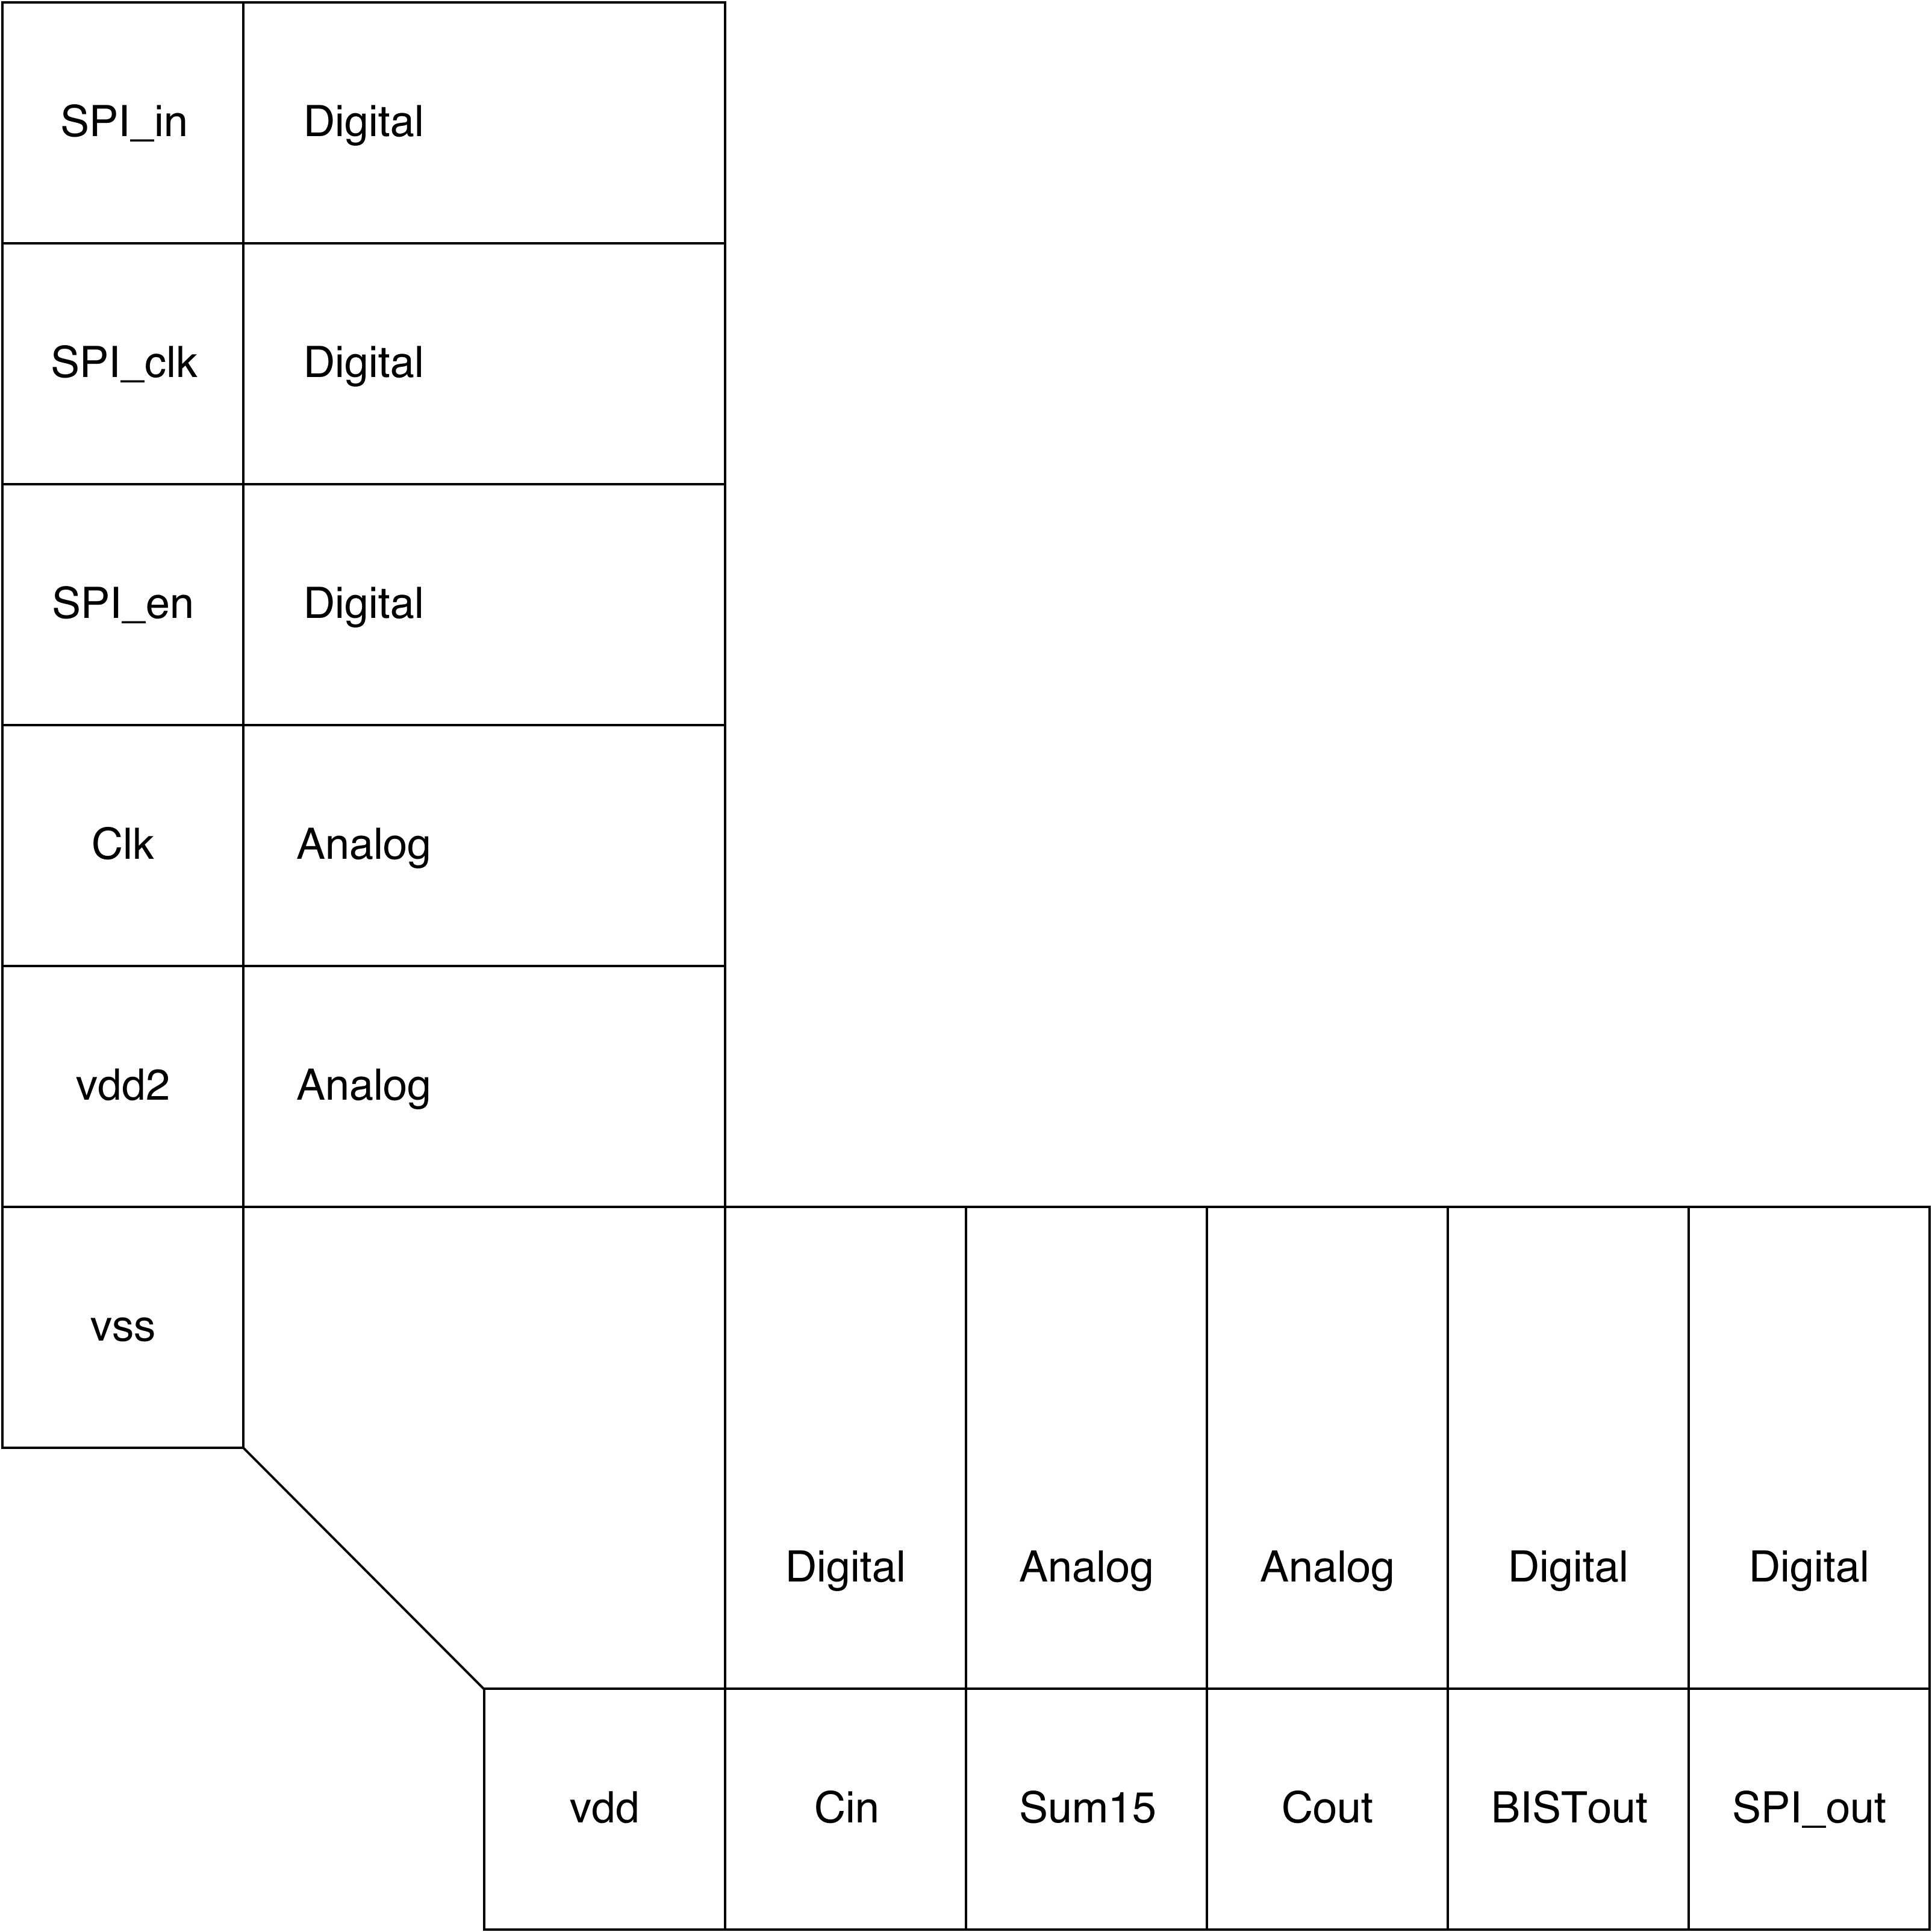
\includegraphics[scale=0.1]{../figures/padframe.png}
\caption{Pad frame showing how to connect things.} \label{fig:padframe}
\end{figure}

               

\subsection{Evaluation}
Tab. \ref{tab:test_data} shows the data that should be fed into the chip to test it's functionality.

\begin{table}[H]
  \caption{Test data}
  \centering
  \begin{tabularx}{\linewidth}{|X|X|X|X|}
    \hline
    \textbf{A} & \textbf{B} & \textbf{Config bits} & \textbf{Check sum} \\ \hline
    1101000110010010 & 1101100100011000 & 0000000000000010 & 1010101010101010\\ \hline
    0100010000110001 & 0001000100100011 & 0000000000000001 & 0101010101010101\\ \hline
    1000000000000000 & 1000000000000000 & 0000000000000111 & 0000000100000001\\ \hline
    1111111111111111 & 1111111111111111 & 0000000000000110 & 1111111111111110\\ \hline
  \end{tabularx}
  \label{tab:test_data}
\end{table}